\documentclass[compress]{beamer}

\usepackage[T1,T2A]{fontenc}
\usepackage[utf8]{inputenc}
\usepackage[english,russian]{babel}
\usepackage{hyperref}
\usepackage{microtype}
\usepackage{csquotes}
\usepackage{amsmath}
\usepackage{amsthm}
\usepackage{amssymb}
\usepackage{mathtext}
\usepackage{physics}
\usepackage{newfloat}
\usepackage{caption}
\usepackage{indentfirst}
\usepackage{hyperref}
\usepackage{mdframed}
\usepackage{graphicx}
\usepackage{subfig}
\usepackage{appendix}
\usepackage{ragged2e} %% for \justifying

%% add hyphenation and word wrap to beamer slides
%% \justifying should explicitely be specified for
%% 'enumerate', 'itemize', etc.
\apptocmd{\frame}{}{\justifying}{}

%% add braces around equation number
\makeatletter
\let\oldtheequation\theequation
\renewcommand\tagform@[1]{\maketag@@@{\ignorespaces#1\unskip\@@italiccorr}}
\renewcommand\theequation{(\oldtheequation)}
\makeatother

%% workaround for the \@ifundefined macro update in the 2018 LaTeX release
%% should be fixed in one of the next releases of caption.sty
\makeatletter
\let\@@magyar@captionfix\relax
\makeatother

\DeclareGraphicsExtensions{.pdf,.png,.jpg,.PNG}
\graphicspath{{./img/}}
\captionsetup[figure]{justification=centering}
\renewcommand{\thesubfigure}{\asbuk{subfigure}}
\DeclareCaptionLabelSeparator{dotseparator}{. }
\captionsetup{labelsep=dotseparator}
\makeatletter\appto{\appendices}{\def\Hy@chapapp{Appendix}}\makeatother
\renewcommand{\appendixtocname}{Приложения}
\renewcommand{\appendixpagename}{Приложения}

\setbeamertemplate{background canvas}[vertical shading][bottom=red!2,top=green!2]

\usetheme{Ilmenau}
\usecolortheme{spruce}
\usefonttheme[onlysmall]{serif}

\setbeamercolor{title in head/foot}{parent=palette primary}
\setbeamercolor{author in head/foot}{parent=palette primary}
\setbeamercolor{institute in head/foot}{parent=palette primary}

\setbeamercolor{title}{fg=black}
\setbeamercolor{frametitle}{fg=black}
\setbeamercolor*{enumerate item}{fg=black}

\setbeamercolor*{bibliography item}{fg=black}
\setbeamercolor*{bibliography entry title}{fg=black}
\setbeamercolor*{bibliography entry author}{fg=black}
\setbeamercolor*{bibliography entry location}{fg=black}
\setbeamercolor*{bibliography entry note}{fg=black}

\setbeamertemplate{enumerate item}[default]
\setbeamertemplate{bibliography entry title}{}
\setbeamertemplate{bibliography entry location}{}
\setbeamertemplate{bibliography entry note}{}
\setbeamertemplate{bibliography item}{\insertbiblabel}

\addtobeamertemplate{navigation symbols}{}{%
    \usebeamerfont{footline}%
    \usebeamercolor[fg]{title}%
    \hspace{1em}%
    \insertframenumber/\inserttotalframenumber
}

\hypersetup{
    colorlinks,
    citecolor=black,
    filecolor=black,
    linkcolor=black,
    urlcolor=black
}

\AtBeginSection[]{
  \begin{frame}
  \vfill
  \centering
  \begin{beamercolorbox}[sep=8pt,center,shadow=true,rounded=true]{title}
    \usebeamerfont{title}\insertsection\par%
  \end{beamercolorbox}
  \vfill
  \end{frame}
}


\deftranslation[to=russian]{Theorem}{Теорема}
\deftranslation[to=russian]{theorem}{Теорема}

\title{Обратные задачи. Тема 1. Вопросы 4--6}
\author{Василевский~А.В.}
\institute[ННГУ]{Нижегородский университет им. Н.И.~Лобачевского}
\date{2019}

\begin{document}

    \frame[plain]{\titlepage}

    \section[Вопрос 4]{Вопрос 4. Экстремальные задачи для выпуклого функционала}

    \begin{frame}\frametitle{Выпуклая функция}

        Выпуклой называется функция (функционал) $f(x)$, удовлетворяющая неравенству (Йенсена):
        %
        \begin{equation*}
            f(\alpha x + \beta y) \le \alpha f(x) + \beta f(y), \qquad \alpha + \beta = 1, \quad \alpha, \beta \ge 0
        \end{equation*}

        Это определение эквивалентно следующему: \enquote{Любая подозрительная на экстремум (минимум) точка является точкой глобального экстремума (минимума)}. Это легко показать:
        %
        \begin{gather*}
            \qquad \alpha = 1 - \beta, \quad f'(x) = 0, \quad \beta \to 0; \\
            \frac{f(x + \beta(x - y)) - f(x)}{\beta} \le f(y) - f(x); \\
            (x - y) f'(x) \le f(y) - f(x); \quad\Longrightarrow\quad \forall y: f(x) \le f(y) \quad\blacksquare
        \end{gather*}

    \end{frame}

    \begin{frame}\frametitle{Строго выпуклая функция}

        Если исходное неравенство при $x \neq y$ строгое, функция называется строго выпуклой.

        Для такой функции верно
        %
        \begin{equation*}
            f'(x) = 0 \quad\longrightarrow\quad \forall y: f(x) < f(y)
        \end{equation*}

        Наличие единственного глобального = локального минимума существенно упрощает численную минимизацию функции, поскольку алгоритм гарантированно сойдется к нужной точке.

    \end{frame}

    \begin{frame}\frametitle{Условная оптимизация}

        Для произвольной функции задача условной оптимизации функции $f(x_i)$ при наличии ограничений $\phi_j(x_i) = 0$ может быть сформулирована как задача оптимизации функции Лагранжа по переменным $x_i \cup \lambda_j$:
        %
        \begin{equation*}
            \mathcal{L}[f;\phi_j](x_i,\lambda_j) =
                f(x_i) + \sum\limits_j \lambda_j \phi_j(x_i) \to \mathrm{opt}_{x_i,\lambda_j}
        \end{equation*}

        Если $f$~--- выпуклая функция, то $\mathcal{L}$ выпукла, если все $\phi_j$ также являются выпуклыми функциями. Причем $\mathcal{L}$ строго выпукла, если все $f$ и $\phi$ также строго выпуклы.

    \end{frame}

    \begin{frame}\frametitle{Выпуклые множества}

        Множество $C$ называется выпуклым, если
        %
        \begin{equation*}
            \forall x,y \in C: \alpha x + \beta y \in C
        \end{equation*}

        Свойства элементов множества $C$ те же, что и у выпуклых функций~--- существует единственный элемент $x_0$, являющийся \enquote{локальным минимумом} множества:
        %
        \begin{equation*}
            \exists! x_0 \in C : \forall x \in C: \inf\limits_{z \in C}{\norm{x - z}} = \norm{x - x_0}
        \end{equation*}

        Пересечение выпуклых множеств~--- также выпуклое множество.

    \end{frame}

    \begin{frame}\frametitle{Операторы проекции}

        Введем оператор проекции на выпуклое множество $C \subseteq F$, $\mathcal{P}_{C}: F \to C$. Определенный таким образом оператор всегда является нерасширяющим. Для строго сужающего оператора тождество
        %
        \begin{equation*}
            x_0 = \mathcal{P} x_0,
        \end{equation*}
        %
        где $x_0$~--- фиксированная точка отображения $\mathcal{P}$, определяет итерационную схему решения задачи с ограничениями:
        %
        \begin{equation*}
            x^{(k+1)} = \mathcal{P} x^{(k)} = \mathcal{P}_n \cdots \mathcal{P}_1 \mathcal{F} x^{(k)} .
        \end{equation*}
        %
        Здесь $\mathcal{F}$~--- некоторый произвольный оператор (функция), а $\mathcal{P}_i$~--- операторы ограничения, хотя бы один из которых строго сужающий.

    \end{frame}

    \section[Вопрос 5]{Вопрос 5. Обратные задачи математической физики, задачи гомографии, обратные задачи для дифференциальных уравнений}

    \begin{frame}\frametitle{Обратные задачи в теории систем}

        \begin{columns}
            \column{0.38\linewidth}
                \centering
                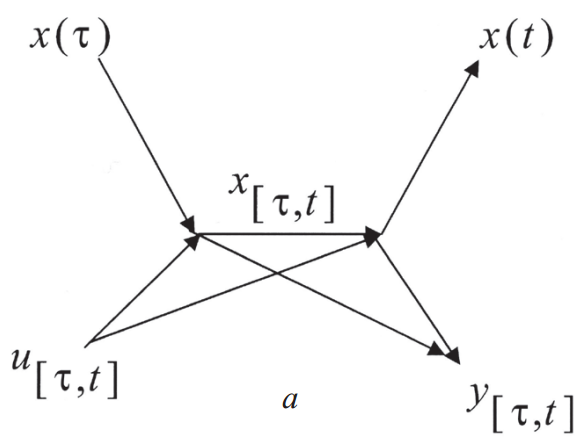
\includegraphics[width=0.9\textwidth]{state_diagram.png}
            \column{0.58\linewidth}
                В.Т.~Борухов и др. \cite{BGT09} дают классификацию обратных задач, возникающих в теории систем. Задачи формулируются путем обращения естественных причинно-следственных связей в динамической системе.
        \end{columns}

        \vspace*{\fill}

        Здесь $x(t)$~--- внутреннее состояние системы, $y(t)$~--- ее наблюдаемое состояние (выходы), $u(t)$~--- внешние воздействия (входы). Индексы $[\tau,t]$ означают действие в пределах указанного отрезка времени.

    \end{frame}

    \begin{frame}\frametitle{Обратные задачи в теории систем}

        Например, автономная линейная система с сосредоточенными параметрами задается в виде:
        %
        \begin{align*}
            \dot{x}(t) &= A x(t) + B u(t) \\
            y(t)       &= C x(t) + D u(t) \\
        \end{align*}

        Обратные задачи: определение коэффициентов $A,\,B,\,C,\,D$, прошлого по будущему.

    \end{frame}

    \begin{frame}\frametitle{Обратные задачи в теории систем}

        Каждая обратная задача может быть сформулирована либо как задача наблюдения (задача восстановления причин по наблюдаемым следствиям), либо как задача управления (синтез причин, обусловливающих требуемые следствия):
        %
        \begin{itemize}
            \item $x(t) \to x(\tau)$: восстановление / синтез начального состояния по известному конечному;
            \item $y_{[\tau,t]} \to x(\tau)$~--- восстановления / синтез начального состояния по выходам;
            \item $y_{[\tau,t]} \to u_{[\tau,t]}$~--- восстановление / синтез входов по известным выходам;
            \item Реализация динамической системы~--- синтез переходных характеристик, обеспечивающих желаемые / наблюдаемые выходы / состояния.
        \end{itemize}

    \end{frame}

    \begin{frame}\frametitle{ОЗ для дифференциальных уравнений}

        Рассмотрим простейшее уравнение теплопроводности:
        %
        \begin{equation*}
            \dot{T}(t,x) = q T''(t,x) + f(t,x) .
        \end{equation*}
        %
        Прямой задачей является отыскание распределения температуры $T(t,x)$ для всех $t>0$ при заданных начальных условиях $T(0,x) = v(x)$ и функции $f(t,x)$.
        %
        Если в эксперименте измеряется $T(t,x_0)$, в некоторой точке $x_0$ стержня и возмущающая функция $f(t,x)$~--- неизвестна, можно поставить задачу отыскания $f(t,x)$ (восстановление входов по выходам). При известной $f(t,x)$ может быть поставлена задача восстановления $T(0,x) = v(x)$ по, например, $T(t,x_0)$ (восстановление начального состояния по выходам).

    \end{frame}

    \begin{frame}\frametitle{Задача гомографии}

        Гомография (проективное преобразование)~--- преобразование, переводящее прямые в прямые. В 3D задается матрицей $H_{4\times4}$ в однородных координатах $(x,\,y,\,z,\,w) = w (\hat{x},\,\hat{y},\,\hat{z},\,1)$. Позволяет описывать перспективные искажения объекта, наряду с обычным поворотом, смещением и т.д.:
        %
        \begin{equation*}
            \vb{r}' = H \vb{r} , \qquad \vb{r} = \qty{x,\,y,\,z,\,w} .
        \end{equation*}

        Задача гомографии~--- поиск матрицы $H$ по набору пар точек $(p,q)$ \enquote{исходная--искаженная}:
        %
        \begin{equation*}
            \vb{r}'_i = H \vb{r}_i, \quad\text{или,}\quad
            R'_{4 \times n} = H_{4 \times 4} R_{4 \times n}, \quad
            R = \qty{\vb{r}_0,\dots,\vb{r}_n} .
        \end{equation*}

    \end{frame}

    \begin{frame}\frametitle{Задача гомографии}

        \centering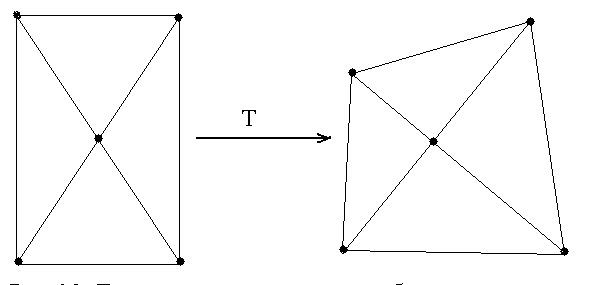
\includegraphics[width=0.9\textwidth]{projective.jpg}

    \end{frame}

    \begin{frame}\frametitle{Задача гомографии}

        Обращая выражение, записанное в матричном виде, получаем:
        %
        \begin{equation*}
            R' = H R \quad\Longrightarrow\quad
            R' R^T = H \qty(R R^T) \quad\Longrightarrow\quad
            H = R' R^T \qty(R R^T)^{-1} .
        \end{equation*}

        Задача некорректно поставлена: не устойчива к шумам и выбросам в данных.

        Другие методы решения:
        %
        \begin{itemize}
            \item Метод максимального правдоподобия (при нормальном распределении шума переходит в МНК).
            \item RANSAC (Random Sample Consensus)~--- стохастический метод (устойчивость к выбросам).
        \end{itemize}

    \end{frame}

    \begin{frame}\frametitle{Задача гомографии}

        Связанные задачи:
        %
        \begin{itemize}
            \item Определение положения калиброванной камеры по проекциям точек;
            \item Определение положения точки по ее проекциям на камеры;
            \item Калибровка камеры по проекциям точек и т.д.
        \end{itemize}

    \end{frame}

    \section[Вопрос 6]{Вопрос 6. Условия корректности обратных задач}

    \begin{frame}\frametitle{Корректность обратных задач}

        Задача называется корректной по Адамару, если ее решение:
        %
        \begin{itemize}
            \item существует;
            \item единственно;
            \item устойчиво (к шумам в входных данных).
        \end{itemize}

        Первое условие обычно предполагается. Отсутствие решения у ОЗ сопряжено, скорее, с неадекватностью выбранной математической модели.

    \end{frame}

    \begin{frame}\frametitle{Единственность решения}

        Условие единственности тесно связано с устойчивостью. Рассмотрим обращение уравнения типа свертки в спектральной области:
        %
        \begin{equation*}
            y = f \circledast x \quad\Longrightarrow\quad
            Y(\omega) = F(\omega) X(\omega) \quad\Longrightarrow\quad
            X(\omega) = \frac{Y(\omega)}{F(\omega)} .
        \end{equation*}
        %
        Из второго уравнения легко видеть, что в области, в которой $F(\omega) = 0$, решение $X(\omega)$ не единственно: $X(\omega)$ может быть выбрана произвольно.

    \end{frame}

    \begin{frame}\frametitle{Устойчивость решения}

        В то же время, если $Y(\omega)$ известно лишь с точностью до шумовой компоненты, в областях, где $F(\omega) \to 0$, шумовые компоненты в решении может бесконечно усиливаться:
        %
        \begin{equation*}
            X(\omega) = \frac{Y(\omega)}{F(\omega)} =
                \frac{Y^*(\omega)}{F(\omega)} + \frac{N(\omega)}{F(\omega)} =
                X^*(\omega) + \frac{N(\omega)}{F(\omega)}
        \end{equation*}

        Рассмотрим СЛАУ вида
        %
        \begin{equation*}
            A \vb{x} = \vb{y} \quad\Longrightarrow\quad
            \vb{x} = A^{-1} \vb{y} = \vb{x}^* + A^{-1} \vb{v} .
        \end{equation*}
        %
        При $\det A = 0$ решение системы не единственно. В то же время, если матрица $A$ получается из эксперимента, легко получить $\det A \approx 0$. Тогда небольшой шум в $\vb{y}$ будет сильно влиять на качество решения.

    \end{frame}

    \section*{Литература}

    \begin{frame}\frametitle{Литература}

        {\tiny{
            \nocite{*}
            \bibliographystyle{abbrv}
            \bibliography{bibliography}
        }}

    \end{frame}

\end{document}
